\documentclass[10 pt]{article}

\usepackage[utf8x]{inputenc}
\usepackage{dsfont}
\usepackage{amsthm}
\usepackage{amsfonts}
\usepackage{tensor}
\usepackage{mathtools}
\usepackage[T1]{fontenc}
%\usepackage[spanish]{babel}
\usepackage[cm]{fullpage}
\usepackage{graphicx}
\usepackage{float}
\usepackage{bm}
\usepackage{setspace}
\usepackage{enumitem}
\usepackage{mdwlist}
\usepackage{parskip}
\usepackage{listings}
\usepackage{color}
%\usepackage{epstopdf}
\usepackage{tikz,datatool}
\usepackage{hyperref}

\newcommand{\HRule}{\rule{\linewidth}{0.5mm}}

\AtBeginDocument{
  \let\myThePage\thepage
  \renewcommand{\thepage}{\oldstylenums{\myThePage}}
}

\newcommand{\gra}{$^\text{o}$}
\newcommand{\dif}{\text{d}}
\newcommand{\avg}[1]{\left\langle #1 \right\rangle}
\newcommand{\ket}[1]{\left| #1 \right\rangle}
\newcommand{\bra}[1]{\left\langle #1 \right|}
\newcommand{\bket}[2]{\left\langle #1 \middle| #2 \right\rangle}
\newcommand{\der}[2]{\frac{\text{d} #1}{\text{d} #2}}
\newcommand{\prt}[2]{\frac{\partial #1}{\partial #2}}
\newcommand{\dert}[3]{\frac{\text{d}^#3 #1}{\text{d} #2^#3}}
\newcommand{\prtt}[3]{\frac{\partial^#3 #1}{\partial #2^#3}}
\newcommand{\dl}{\mathcal{L}}
\newcommand{\dha}{\mathcal{H}}
\newcommand{\vol}{\text{vol}}
\renewcommand{\vec}[1]{\pmb{#1}}

\newenvironment{algo}[1]
{  \begin{center}
   \mbox{
       \begin{minipage}{\textwidth}
           \begin{tabbing}
           \settabs
            #1
           \end{tabbing}
        \end{minipage}
    }
    \end{center}
}{}
\newcommand{\settabs}{mmm\=mmm\=mmm\=mmm\=mmm\=mmm\=\kill}

\DeclarePairedDelimiter\ceil{\lceil}{\rceil}
\DeclarePairedDelimiter\floor{\lfloor}{\rfloor}

\definecolor{mygray}{rgb}{0.4,0.4,0.4}
\definecolor{mygreen}{rgb}{0,0.5,0.25}
\definecolor{myorange}{rgb}{1.0,0.4,0}

\definecolor{clock0}{cmyk}{1,0,0,0}
\definecolor{clock1}{cmyk}{1,1,0,0}
\definecolor{clock2}{cmyk}{0,1,0,0}
\definecolor{clock3}{cmyk}{0,1,1,0}
\definecolor{clock4}{cmyk}{1,0,1,0}
\definecolor{clock5}{cmyk}{1,1,1,0}
\definecolor{clock6}{cmyk}{0,0,1,0}
\definecolor{clock7}{cmyk}{0,0,0,0.1}

\begin{document}

\lstset{
language=C++,
basicstyle=\ttfamily\color{black},
commentstyle=\color{mygray}\ttfamily,
frame=single,
numbers=left,
numbersep=5pt,
numberstyle=\tiny\color{mygray}\ttfamily,
keywordstyle=\color{mygreen}\ttfamily,
showspaces=false,
showstringspaces=false,
stringstyle=\color{myorange}\ttfamily,
tabsize=2,
emph={double,uint8_t,uint16_t,uint32_t,uint64_t,int8_t,int16_t,int32_t,int64_t},
emphstyle={\color{blue}\ttfamily}
}

\begin{center}
  \Large \textsc{Week 2: Random Walks}
\end{center}

\begin{center}
  \large \textsc{Francisco García Flórez}
\end{center}

\section{Introduction}

In this assignment random walks will be studied, both in two and three dimensions. Moreover, we will compute $\avg{R^2(N)}$, that is, the distance squared after each step from the origin averaged over a number of walks and study its functional dependence.


\section{Program usage}

Following there is a brief guide explaining how to use the program:

\begin{itemize}
  \item \texttt{week2 -N int}: computes Pi using \texttt{int} points in a square of size $[-1,1]\times[-1,1]$, counting how many lie inside a circle of radius one.
  \item \texttt{week2 -e float}: calls the previous function with increasingly larger amounts of points until Pi is approximated with an error less than \texttt{float}.
  \item \texttt{week2 -walk dim steps file}: performs a random walk in \texttt{dim} dimensions with \texttt{steps} steps, and saves its results to file in json\footnote{See \url{http://www.w3schools.com/json/} for more information.} format.
  \item \texttt{week2 -pwalk dim steps size file}: performs a random walk just in the previous case, including now periodic boundary conditions as a \texttt{dim}-dimensional box of size \texttt{size}.
  \item \texttt{week2 -rsquared dim steps nwalks file}: performs \texttt{nwalks} random walks computing $\avg{R^2(N)}$ and saving it to \texttt{file}, also in json format.
  \item \texttt{week2 -prsquared dim steps nwalks size file}: similar to the previous function, incorporating now periodic boundary conditions.
\end{itemize}

By running the script \texttt{week2.sh} these commands will be executed, showing their results. By executing \texttt{python python/graphs.py} a number of plots can be generated.

\section{Random walks}

\subsection{Functional dependence of $\avg{R^2(N)}$}

Firstly, we compute the required data by executing the following commands:

\begin{itemize}
  \item \texttt{./bin/week2 -rsquared 2 200 10000 data/rsquared2.json}
  \item \texttt{./bin/week2 -prsquared 2 200 10000 20.0 data/prsquared2.json}
  \item \texttt{./bin/week2 -rsquared 3 200 10000 data/rsquared3.json}
  \item \texttt{./bin/week2 -prsquared 3 200 10000 20.0 data/prsquared3.json}
\end{itemize}

And then, after plotting their results we get:

\begin{figure}[H]
  \begin{center}
    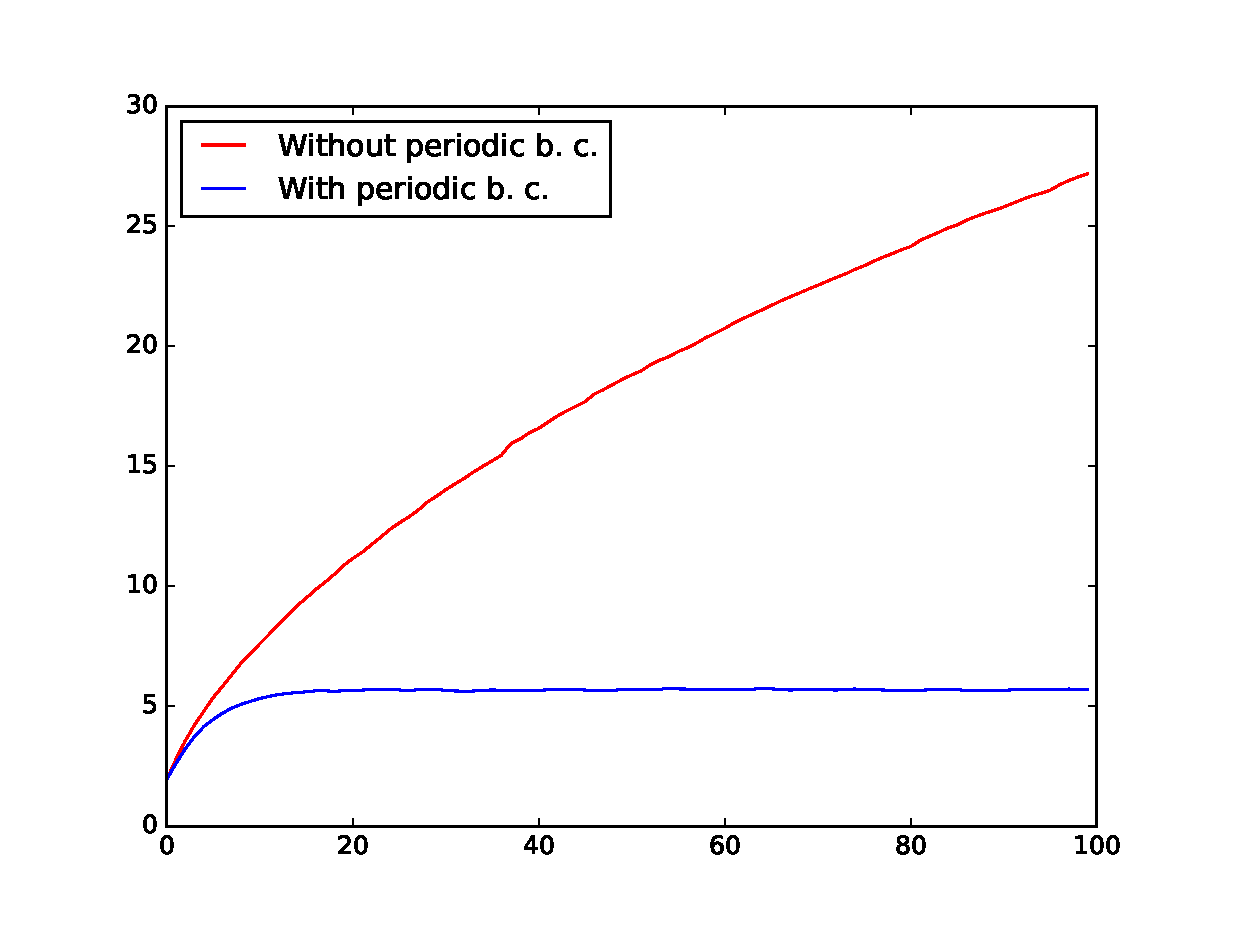
\includegraphics[width=0.6\textwidth]{../graphs/rsquared2.eps}
    \caption{Graphical representation of $\avg{R^2(N)}$ in 2D.}
  \end{center}
\end{figure}

It is easy to spot the linear dependence of $\avg{R^2(N)}$ when there are no periodic boundary conditions (``PBC'' in the following), with a slope of $1.00\pm0.01$ and r-value larger than $0.9999$. In the second case, with PBC, fitting the function doesn't look that easy. At least, we can see that instead of increasing uncontrollably, it is bounded by some limit value.

If we fit the data to $f(x) = a(1-e^{-bx})$, even if it's not perfect, allows us to estimate $a \sim 70$ in this case. This behavior is expected, however, since the particle cannot escape the box. It is also expected that up to some number of steps $N_*$ both averages should take almost the same value, namely, when the probability of reaching the boundary is not negligible.

A better fitting function may be a hyperbole, $ax^2 - by^2 = c$, rotated so the axis match with the unbounded line and the limit, blue and magenta lines respectively.

Now, repeating this procedure for three dimensions we get the following results:

\begin{figure}[H]
  \begin{center}
    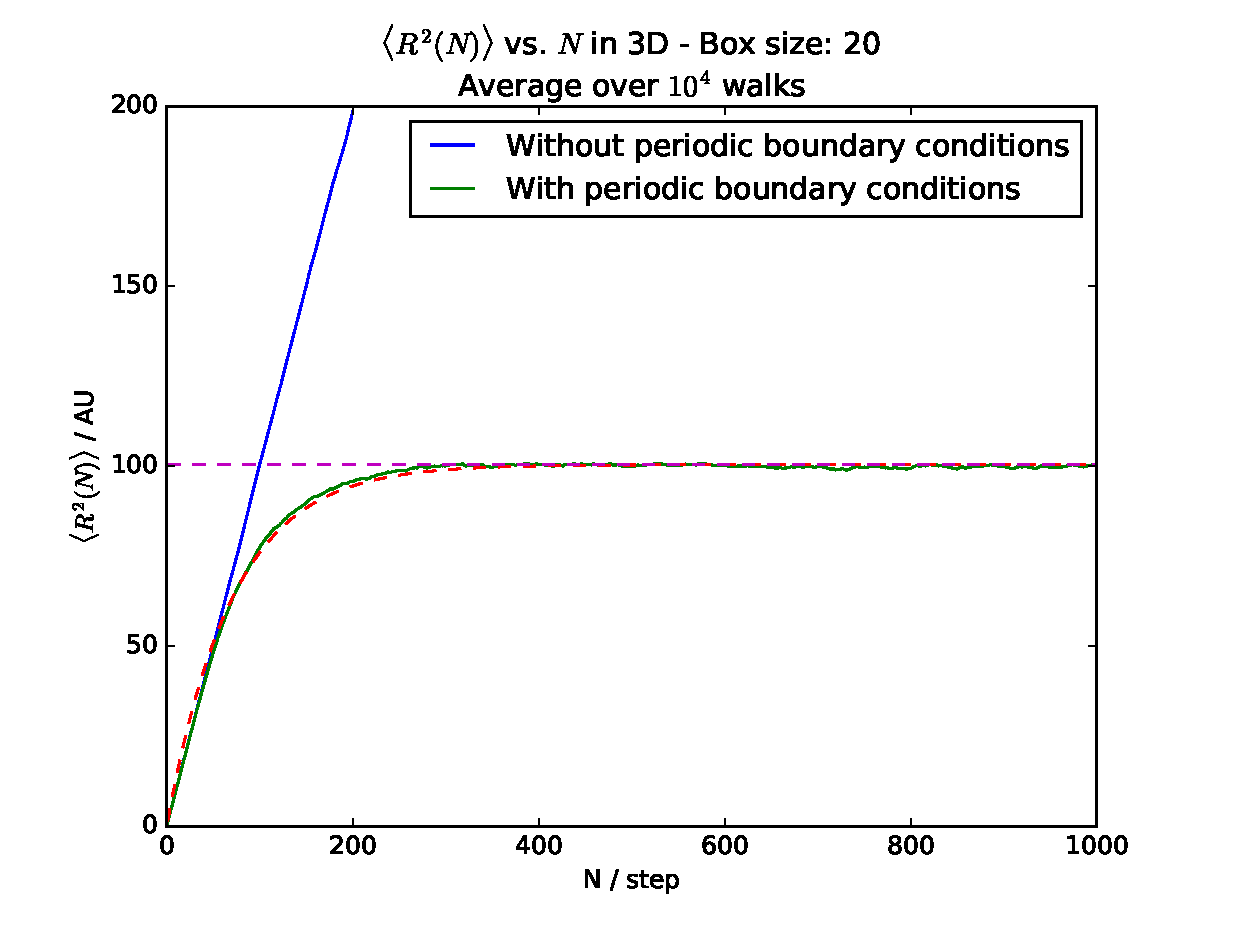
\includegraphics[width=0.6\textwidth]{../graphs/rsquared3.eps}
    \caption{Graphical representation of $\avg{R^2(N)}$ in 3D.}
  \end{center}
\end{figure}

So, the linear dependence of $\avg{R^2(N)}$ in the unbounded case has not changed, however considering PBC the limit of $N \rightarrow \infty$ changes to $a \sim 110$. This increase makes sense after all, since in 3D the particle has more ``freedom'' to move around before getting to the borders, and therefore this average will be closer to the unbounded case. It is also possible to interpret this result by considering that the surface of a sphere in 3D is larger ($4\pi$ against $2\pi$) than its two dimensional counterpart, so the probability of concatenating several steps in the same direction is lower.

As an experiment, the following results were generated from random walks in 1D and 11D, so this dimension dependent behavior is more explicit:

\begin{figure}[H]
  \begin{center}
    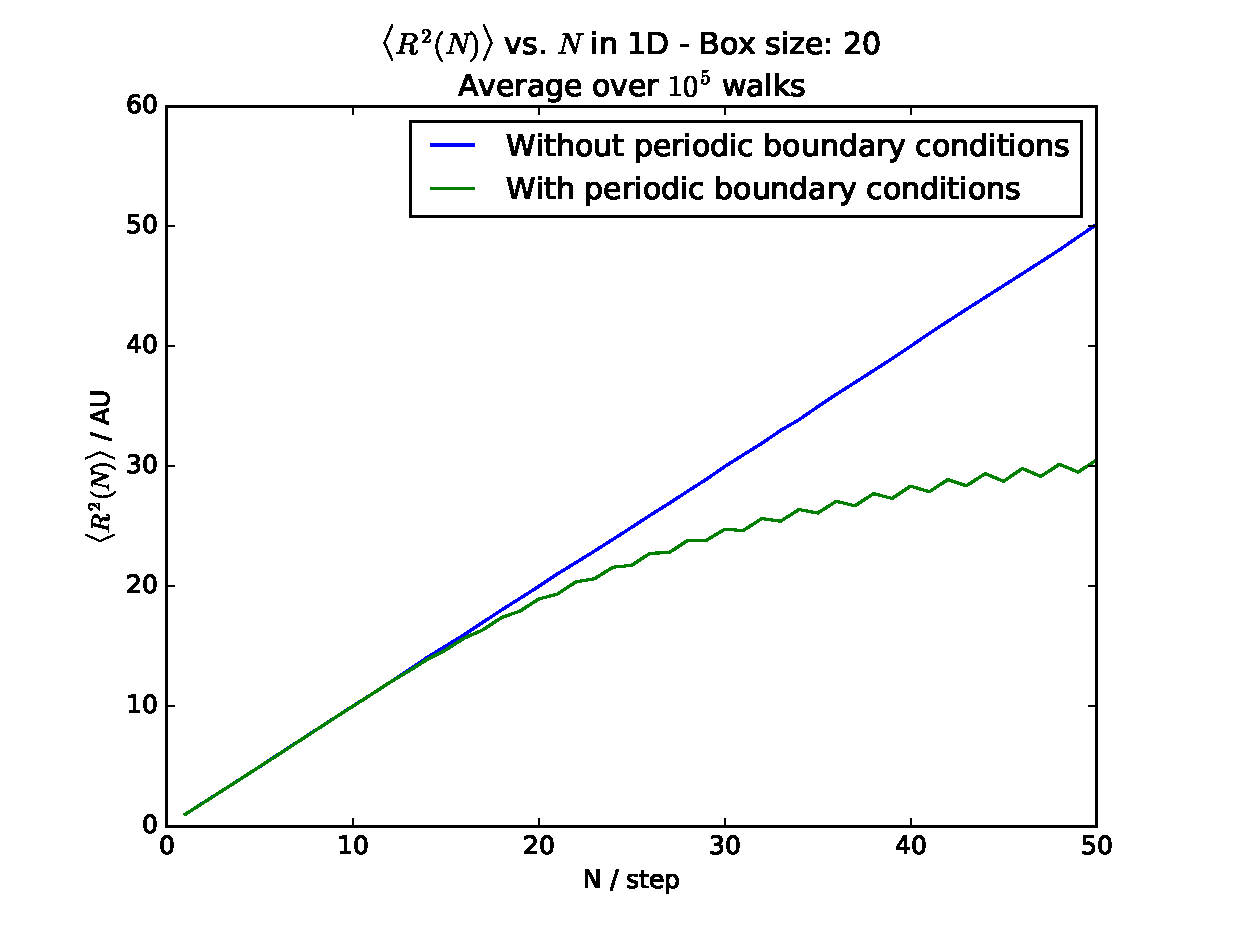
\includegraphics[width=0.45\textwidth]{../graphs/rsquared1.eps}
    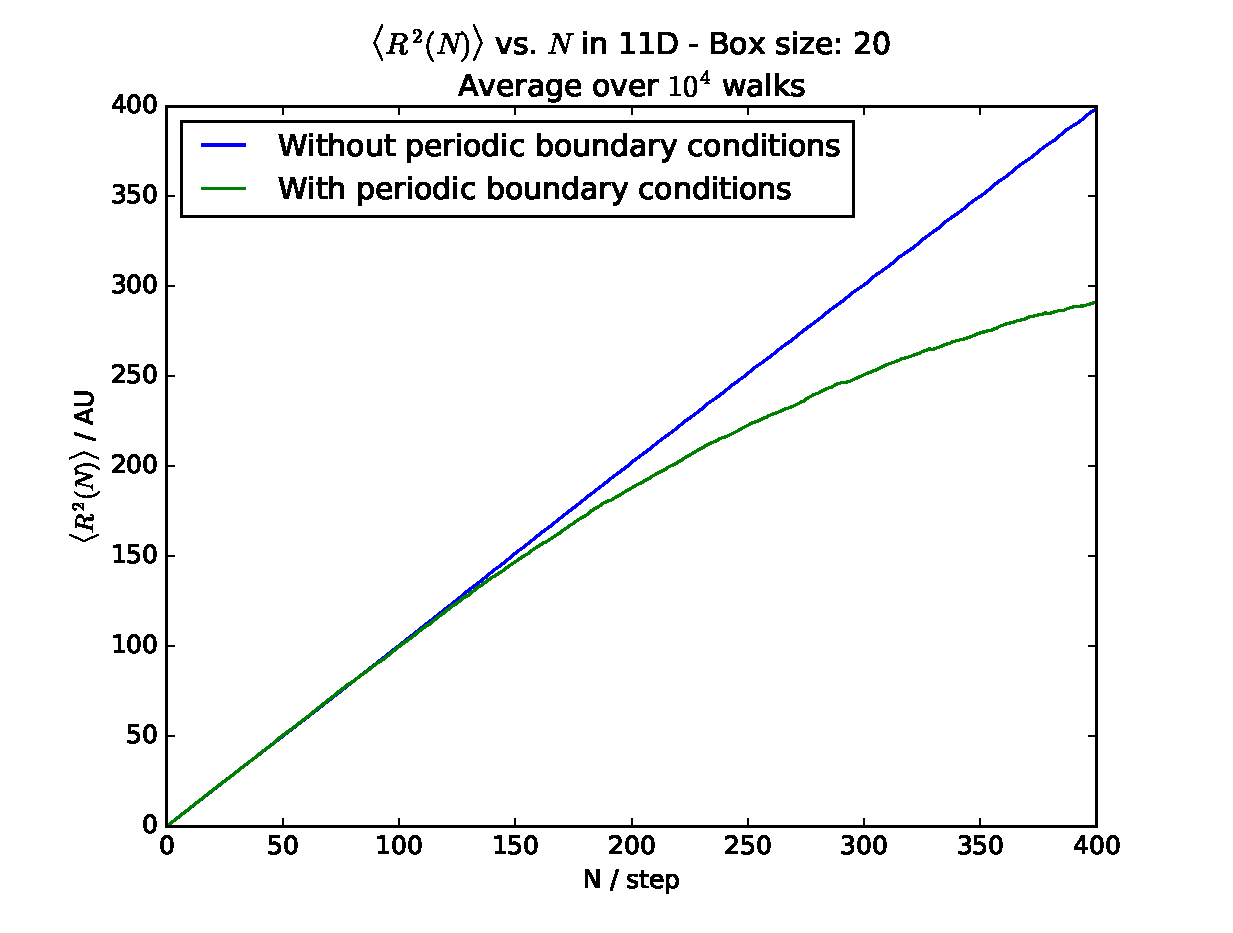
\includegraphics[width=0.45\textwidth]{../graphs/rsquared11.eps}
    \caption{Graphical representation of $\avg{R^2(N)}$ in 1D and 11D.}
  \end{center}
\end{figure}

As expected, in 1D $a$ is lower than in the previous cases, at it reaches the limit quicker. Although, we can easily see some unexpected behavior: ``steps'' in the function when imposing PBC. This may be explained by considering that in 1D one step can only by taken in two different directions, with 50\% chance for each, so it may produce this effect. In 11D on the other hand, everything works as expected, with a larger value for $a$ and smaller for $b$.

\subsection{Generating random unit vectors}

If we tried to generate uniformly distributed points on the surface of a sphere by choosing two random values for the angles, we wouldn't find a uniform distribution on the surface. It's easy to visualize by mapping uniformly chosen points from $[0,\pi]\times[0,2\pi]$ to the sphere, as most of them will be located near the poles.

Instead of using a uniform probability distribution for generating random numbers in angle-space, it would be possible to choose a different one that compensates this spherical deformation. However, not easily done.

Since we cannot check uniformity by only looking at plots like the following, we have to follow a more indirect procedure.

\begin{figure}[H]
  \begin{center}
    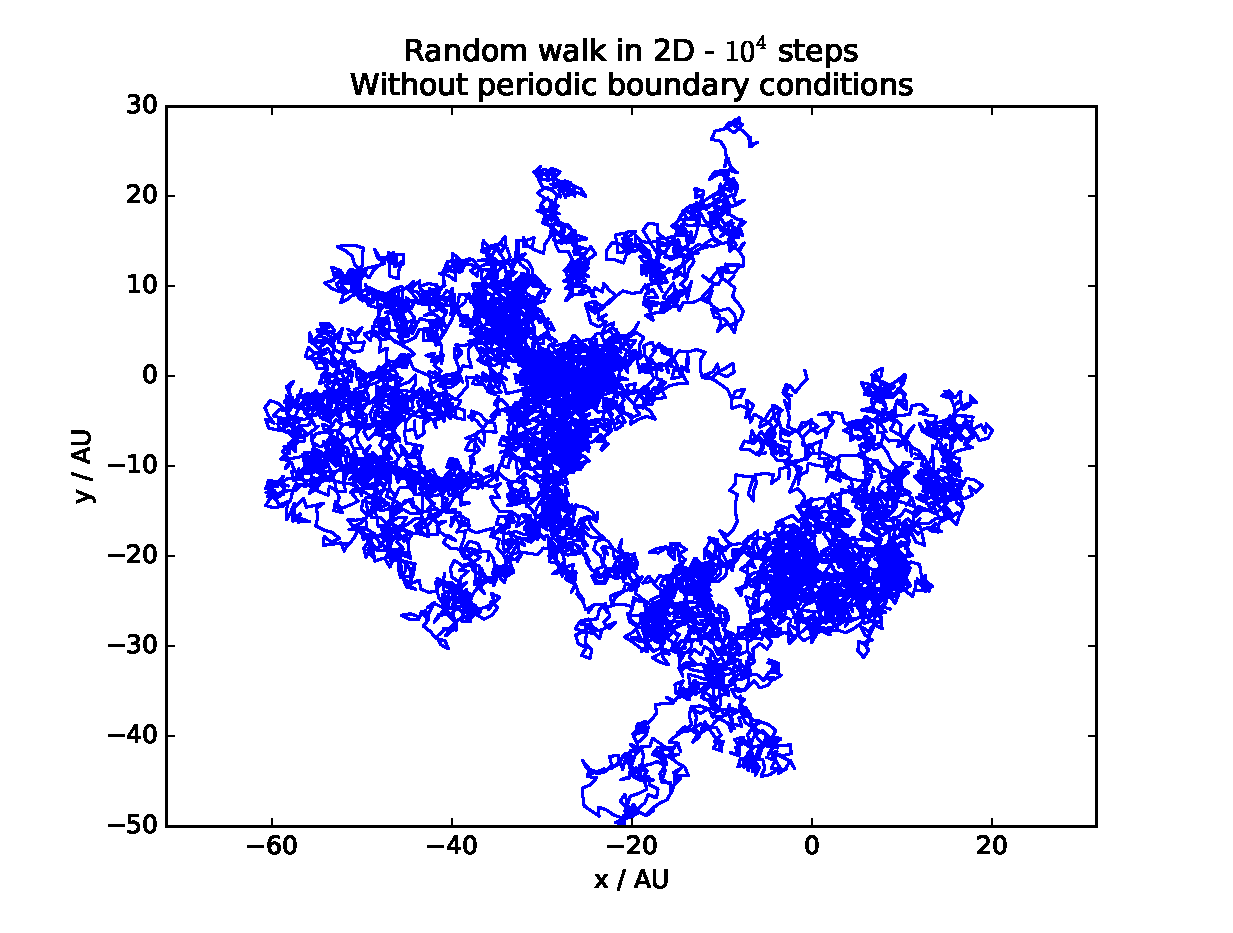
\includegraphics[width=0.45\textwidth]{../graphs/randomwalk2.eps}
    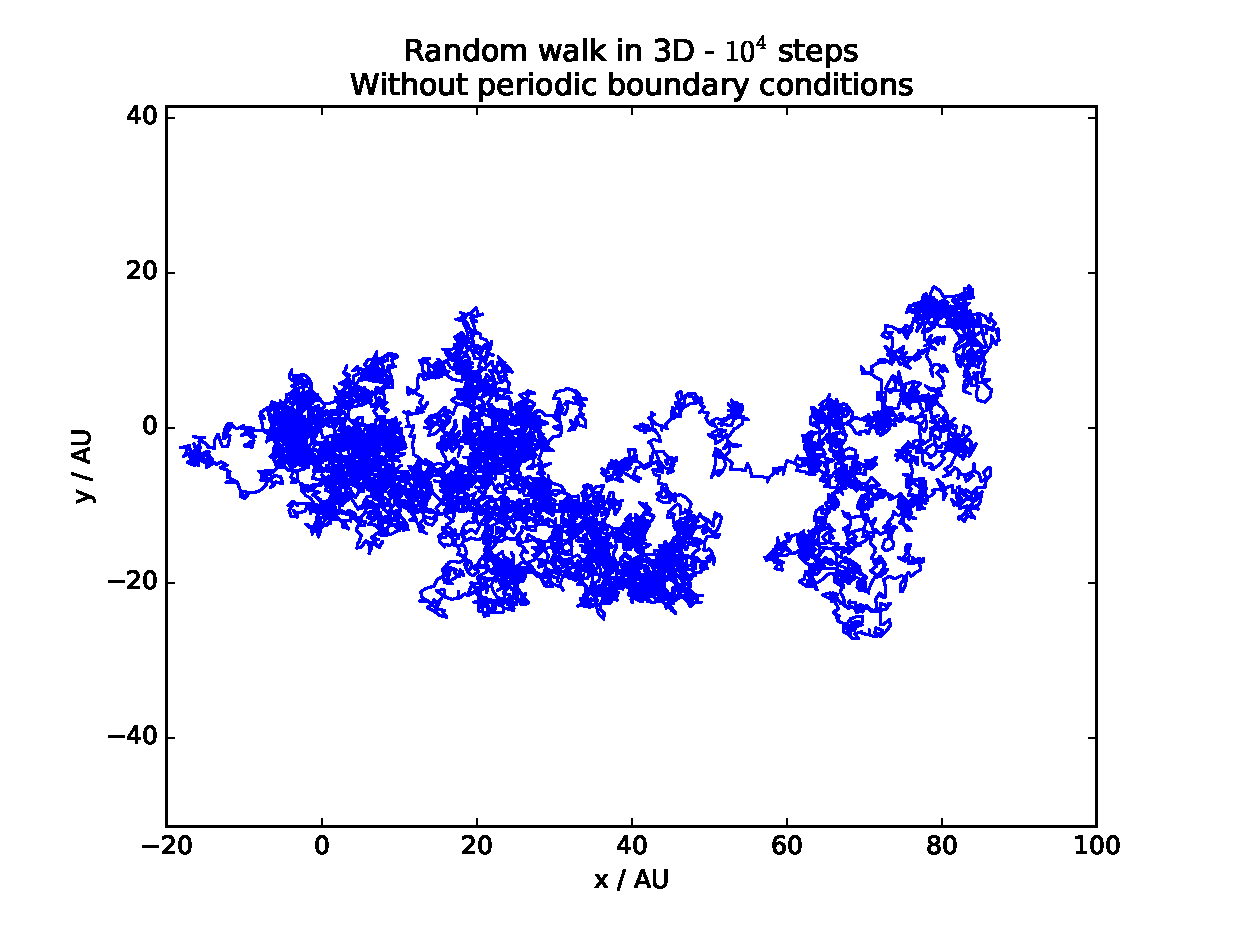
\includegraphics[width=0.45\textwidth]{../graphs/randomwalk3.eps}
    \caption{Graphical representation of a random walk in (left) 2D and (right) 3D projected to a plane.}
  \end{center}
\end{figure}

For example, considering only random walks of $N_S$ steps, we can make a density plot of how many times each point has been visited. When there are no bounds, we expect that for $N_S$ large enough, this density distribution will have rotational invariance. In the following plot the results are represented:

\begin{figure}[H]
  \begin{center}
    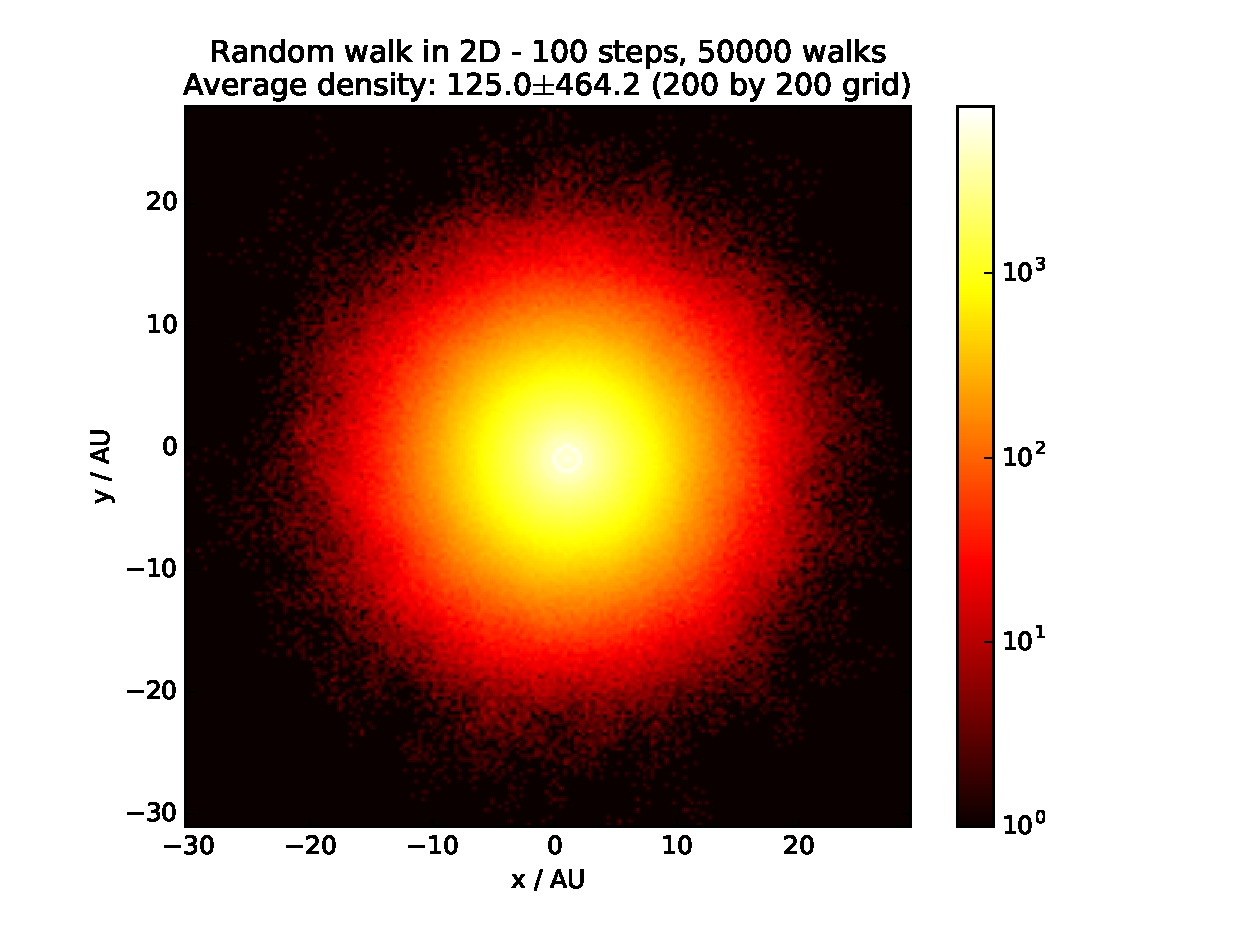
\includegraphics[width=0.45\textwidth]{../graphs/randomwalk2map.eps}
    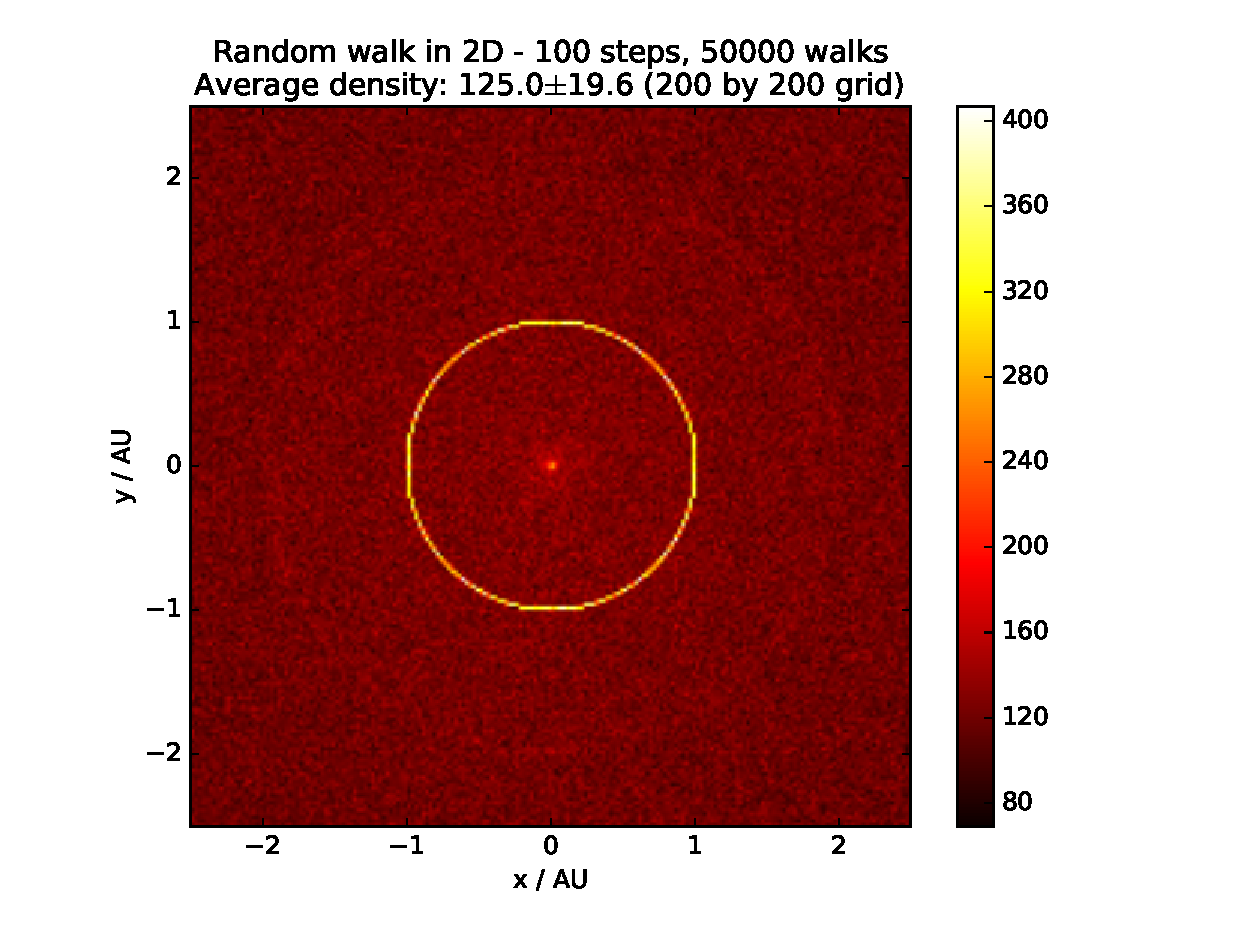
\includegraphics[width=0.45\textwidth]{../graphs/prandomwalk2map-b.eps}
    \caption{Density distribution of visited points in 2D. (left) Without boundary conditions, (right) with periodic boundary conditions.}
  \end{center}
\end{figure}

It's clear, even more so in the right plot, that our vectors are indeed uniformly distributed in the sphere. In this case we have performed the random walk in 2D, but the algorithm for generating the next step is the same independently of dimensions.

On the other hand, we can also analyze a similar density distribution generated this time by only one walk after a large number of steps:

\begin{figure}[H]
  \begin{center}
    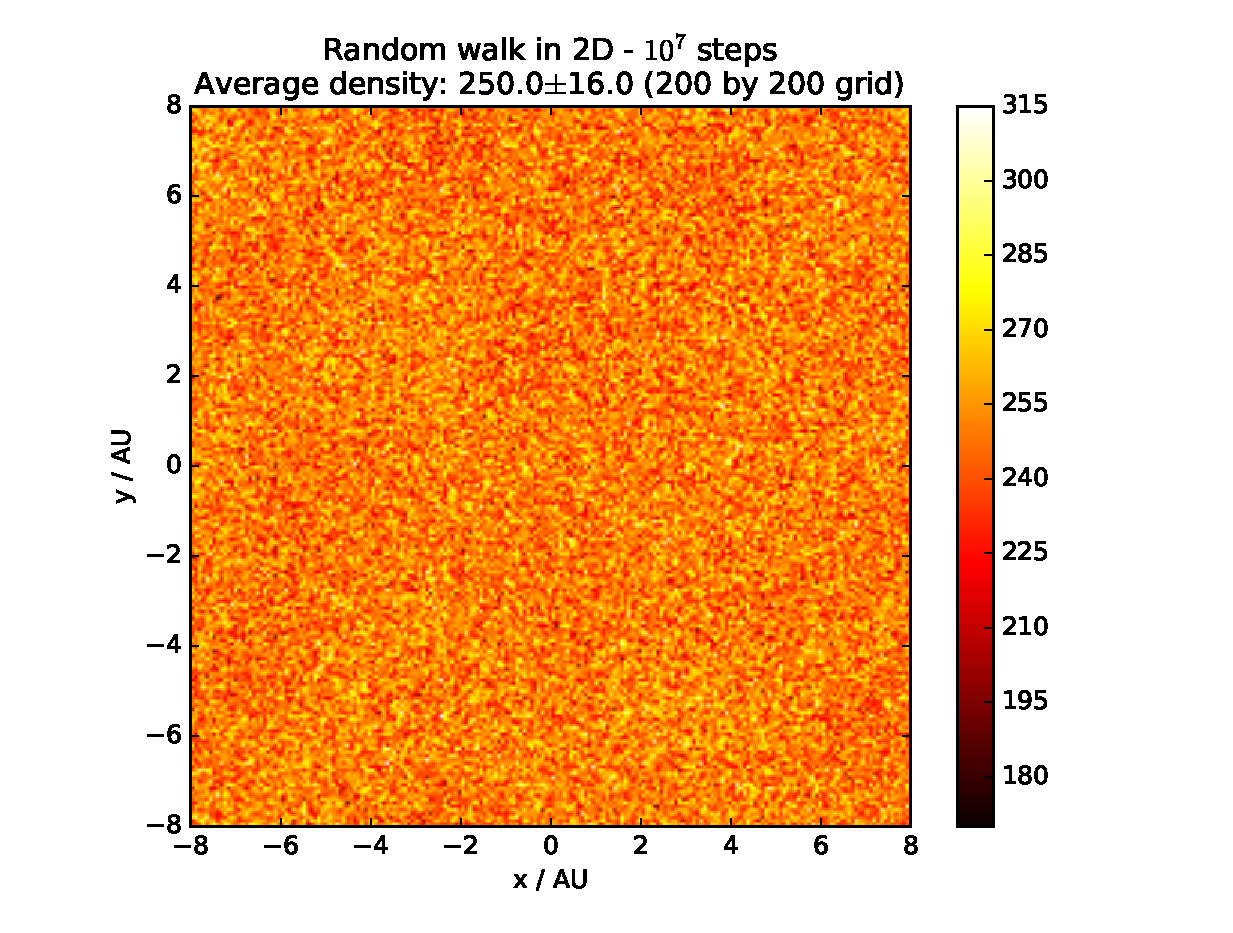
\includegraphics[width=0.6\textwidth]{../graphs/prandomwalk2map.eps}
    \caption{Density distribution of points visited by one random walk with periodic boundary conditions.}
  \end{center}
\end{figure}

As expected this distribution is uniform, with small fluctuations around the average. Although, an histogram of the probability density around this average shows something a bit unexpected:

\begin{figure}[H]
  \begin{center}
    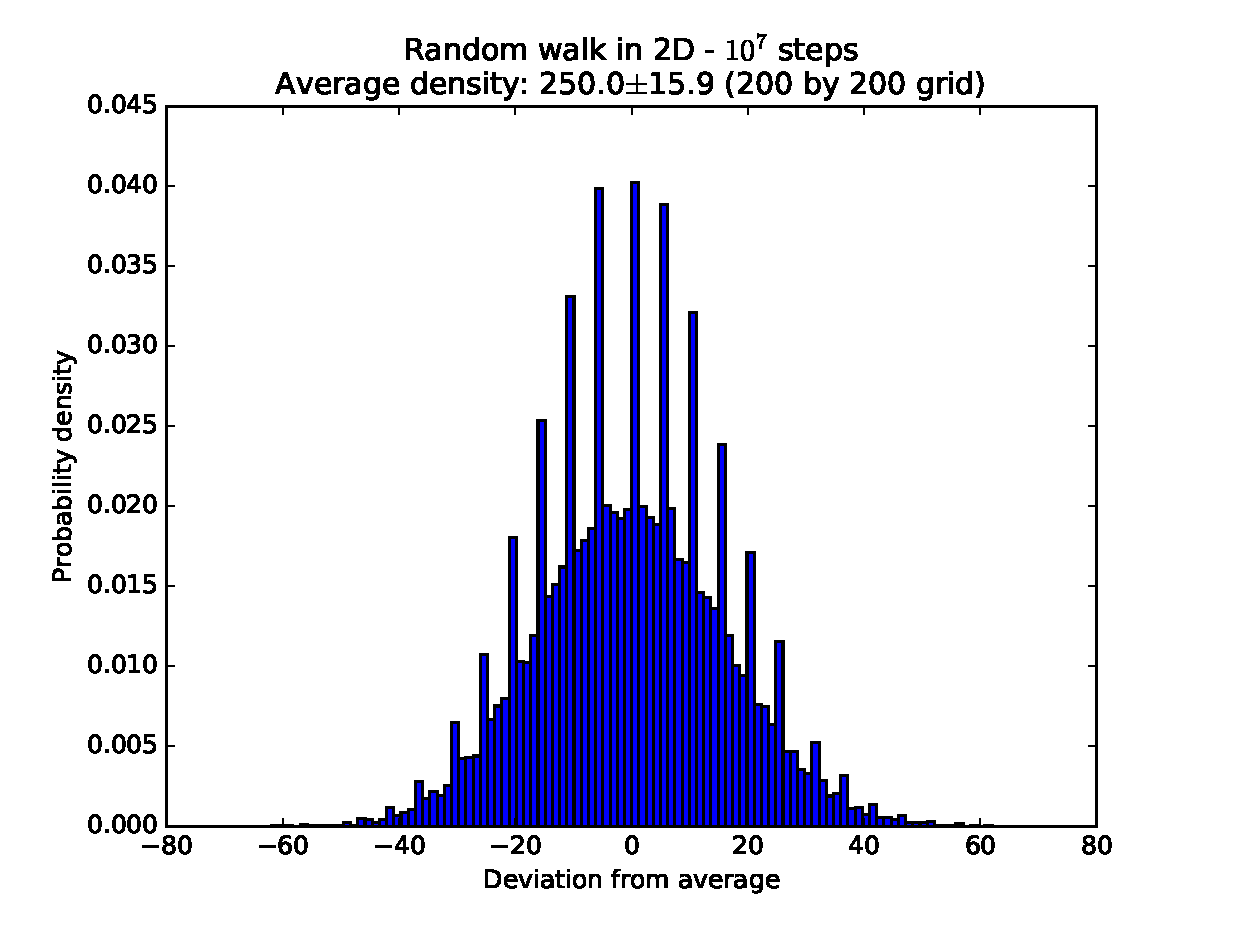
\includegraphics[width=0.6\textwidth]{../graphs/prandomwalk2-hist.eps}
    \caption{Distribution of values around the average.}
  \end{center}
\end{figure}

Of course, those fluctuations are Gaussian around the average, but it seems like there are two different sources, generating two clearly different distributions. This behavior is not dependent on the box size, and as of now the possible reasons behind it are not clear.

\end{document}
